% filename: HEP_GL_IPZ_OSS_Coldflow_OperationSafetyConcept

\documentclass{article}

\usepackage[utf8]{inputenc}
\usepackage[top=3cm, headheight=2.2cm, headsep=10pt]{geometry}
\usepackage{graphicx}

% To reference the last page
\usepackage{lastpage}

% Like `tabularx` but supports pagebreaks
\usepackage{ltablex}
% Adjust row vertical spacing
\renewcommand{\arraystretch}{1.2}

% Multiline cells
\usepackage{makecell}

% Set date format to ISO 8601
\usepackage{datetime}
\newdateformat{isodate}{\THEYEAR-\twodigit{\THEMONTH}-\twodigit{\THEDAY}}

% Table colouring
\usepackage[table,dvipsnames]{xcolor}
\definecolor{tableHeaderColor}
{rgb}{0.75,0.75,0.75}
\definecolor{tableColumnColor}
{rgb}{0.95, 0.95, 0.95}
\definecolor{notesColor}
{rgb}{0.95, 0.95, 0.95}
\definecolor{highlightColor}
{rgb}{1.00, 0.95, 0.80}

% Icons for checkbox
\usepackage{pifont}

% Command to create a checkbox
\newcommand{\checkbox}{\ding{113}}

% For automatic counters
\usepackage{array}

% Header and footer
\usepackage{fancyhdr}
\pagestyle{fancy}
\fancyhf{} % Clear header and footer
\renewcommand{\headrulewidth}{0pt}
\lhead{\includegraphics[width=2cm]{../../common/assets/HELIOS_LOGO.png}}
\rhead{\includegraphics[width=2cm]{../../common/assets/ARIS_space_to_grow_LOGO-black.pdf}}
\cfoot{\thepage}
\fancyfoot[L]{Project HEPHAESTUS}
\fancyfoot[C]{Page \thepage\ out of \pageref{LastPage}}

% Draft watermark
\newboolean{isDraft}
\setboolean{isDraft}{true} % Set to false to remove the watermark
\ifthenelse{\boolean{isDraft}}{
  \usepackage{background}
  \backgroundsetup{
    scale=25,
    color=gray,
    opacity=0.4,
    angle=45,
    position=current page.center,
    contents={Draft}
  }
}{}

% Highlight colour
\usepackage{soul}
\sethlcolor{magenta}

% Strikethrough
\usepackage[normalem]{ulem}

% Clickable Hyperlinks
\usepackage[colorlinks=true, linkcolor=blue, urlcolor=blue]{hyperref}

% Toggleable procedure items
\usepackage{etoolbox}



\title{IPZ OSS Coldflow Operation Safety Concept}
\author{Guideline}
\date{Version: \isodate\today}

\begin{document}

\maketitle

% Set the page style for the title page
\thispagestyle{fancy}

\section{Scope}

Within the framework of the ETH Focus Project HEPHAESTUS, Oxidizer Supply System (OSS) cold flows will be performed on the IPZ area. The purpose of a cold flow is to inject only one of the propellants without ignition, to check if the propellant supply system functions correctly under operating conditions.  
\noindent
For the OSS cold flow \textbf{Liquid Oxygen} will be used. To ensure efficient and safe tests, this operational safety concept shall describe the test area and its available safety equipment, gives instructions on how to behave during procedures and in emergencies and analyses the major risks associated with this test as well as the protection mechanisms in place.

\section{Location of safety-relevant Institutions}
The contact information of the relevant safety institutions is listed in \ref{tab:safety-relevant-institutions}.
\begin{table}[h]
    \caption{Information of safety-relevant institutions}
    \label{tab:safety-relevant-institutions}
    \begin{tabularx}{0.9\textwidth}{|X|X|X|}
        \hline
        \rowcolor{tableHeaderColor} \textbf{Description} & \textbf{Address} & \textbf{Phone Number} \\ \hline
        Test Location & \begin{minipage}[t]{\linewidth}
            Innovationspark Zürich \\
            Wangenstrasse 68 \\
            8600 Dübendorf
            \vspace{1mm}
        \end{minipage} & +41 44 527 20 20 \\ \hline
        Spital Uster & \begin{minipage}[t]{\linewidth}
            Brunnenstrasse 42 \\
            8610 Uster
            \vspace{1mm}
        \end{minipage} & +41 44 911 11 11 \\ \hline
        President ARIS & Chloé Pilloud & +41 79 226 39 42 \\ \hline
        Technical Advisor & Bruno Berger & +41 79 209 39 27 \\ \hline
    \end{tabularx}
\end{table}
\noindent
In table \ref{tab:emergency-numbers} the emergency numbers are listed. Call them first before calling other relevant security institutions. In the case of an emergency, follow the contingency procedures as described in Section \ref{emergency-behaviour}.
\begin{table}[h]
    \caption{Emergency Numbers}
    \label{tab:emergency-numbers}
    \begin{tabularx}{0.9\textwidth}{|X|X|}
        \hline
        \rowcolor{tableHeaderColor} \textbf{Description} & \textbf{Phone Number} \\ \hline
        Ambulance & 144 \\ \hline
        Rega & 1414 \\ \hline
        Fire service & 118 \\ \hline
        Police & 117 \\ \hline
        Toxics & 145 \\ \hline
    \end{tabularx}
\end{table}
\newpage
\section{Risk Analysis}
Liquid Oxygen Coldflows involve pressurized systems and therefore have an inherent risk. Additionally, the strong oxidizing properties and cryogenic state of liquid oxygen pose further challenges. The risks associated with these tests are:
\subsection{Overpressure}
An overpressure of the system can lead to rupture of components and therefore to an explosion. Overpressure can cause injury to personnel, namely hearing damage, lung damage and even death, and damage to surrounding facilities. However, during all operations with the trailer, the pressure is limited to 60 bar and all components of the system have previously been tested to 60 bar. Additional preventive measures are taken to minimise the chance of occurance and damage caused by a possible overpressure event:
\begin{itemize}
    \item Every potentially closed section of the system is equipped with a pressure relief valve, which are set to open at 80 bar. This ensures that the pressure in the system is limited to 80 bar, even in the case a pressure reducer were to fail or trapped LOX were to start evaporating. While this is higher than what the components have been tested to on the OSS side, all components are rated for at least 180 bar, which leaves a safety margin against plastic deformation of 2.25.
    \item The TNT equivalent of the potential energy stored in the system and the size of the corresponding safety radius were calculated according to the ASME PCC-2-2018 standard. The safety radius was determined to be 5 meters. To have an additional safety margin and because it's easier to tape off the quadratic test area, the entire test area, which has a radius of around 45 meters, is taped off and monitored during testing.
    \item The system is equipped with multiple pressure sensors which are monitored continuously during testing. If the pressure exceeds the set limit, an automatic abort is triggered which immediately depressurizes the system.
\end{itemize}
\subsection{Asphyxiation}
Asphyxiation can occur if there is a leak of nitrogen gas into the atmosphere. Nitrogen is an inert gas and therefore does not cause any immediate harm to the human body. However, nitrogen displaces oxygen from the air and can therefore lead to asphyxiation. This risk is mitigated by performing the tests outdoors, where the nitrogen can disperse into the atmosphere and does not accumulate.
\subsection{Cryogenic Burns}
Cryogenic burns can occur if a person comes into contact with the cryogenic liquid oxygen. Liquid oxygen has a temperature of -183°C and can cause severe burns on contact with human skin. To prevent this, multiple safety measures are implemented:
\begin{itemize}
    \item All people working on the system during liquid oxgen filling and pressurization are required to wear adequate protective equipment, namely:
    \begin{itemize}
        \item Cryogenic resistant face shield to protect the face from splashes of liquid oxygen
        \item Cryogenic resistant apron to protect the body from splashes of liquid oxygen
        \item Cryogenic resistant gloves to protect the hands from splashes of liquid oxygen
        \item Safety shoes to protect the feet from splashes of liquid oxygen
        \item Thin cotton textiles to avoid saturation with liquid oxygen covered by a nonporous raincoat.
    \end{itemize}
    \item Procedures are in place to avoid personnel standing in areas where liquid oxygen could be released from the system and dry runs are performed to train the procedures.
    \item The safety officer enforces the protected zones around the system during pressurization and liquid oxygen filling.
    \item Finally, the contingency procedures for injury also cover the treatment of cryogenic burns.
\end{itemize}

\subsection{Fire}
The strong oxidizing properties of liquid oxygen can cause fires if it comes into contact with flammable materials. The risk of fire is mitigated by:
\begin{itemize}
    \item All parts of the system that can come into contact with liquid oxygen are made of non flammable, liquid oxygen compatible materials.
    \item The whole OSS section is thoroughly cleaned in accordance with cleaning for oxygen service (CFOS) procedures before the tests.
    \item The system is purged with nitrogen before the tests to remove any particles that could ignite in contact with liquid oxygen.
\end{itemize}

\subsection{Injury}
To conduct the tests, gas bottles have to be handled and moved from the gas storage to the test site. Since the gas bottles are heavy and can be difficult to handle, they pose a risk of injury. To mitigate this risk, all personnel involved in handling the gas bottles are required to wear safety shoes, thick clothing and gloves. Additionally, the gas bottles are transported using a gas bottle trolley to reduce the risk of injury.

\section{Site Map}
The tests will be performed in the IPZ Test Area 2. The trailer will be positioned all the way at the fence to the airfield, with both the side of the system that will be pressurized and the engine compartment facing the airfield. The control station will be positioned close to the Hangar. The whole testing area will be taped off to prevent accidental trespassing and during pressurized operations a dedicated person will monitor the area to look out for trespassers.
Figure \ref{fig:location-plan} shows the setup of the test location and the location of the fire extinguisher and first aid kit. During active testing, only the test conductor, safety officer and engineer in charge are allowed inside the taped zone with appropriate safety equipment (safety goggles and ear protection). When the system is pressurized, no one is allowed inside the taped off safety zone.
\begin{figure}[h]
    \centering
    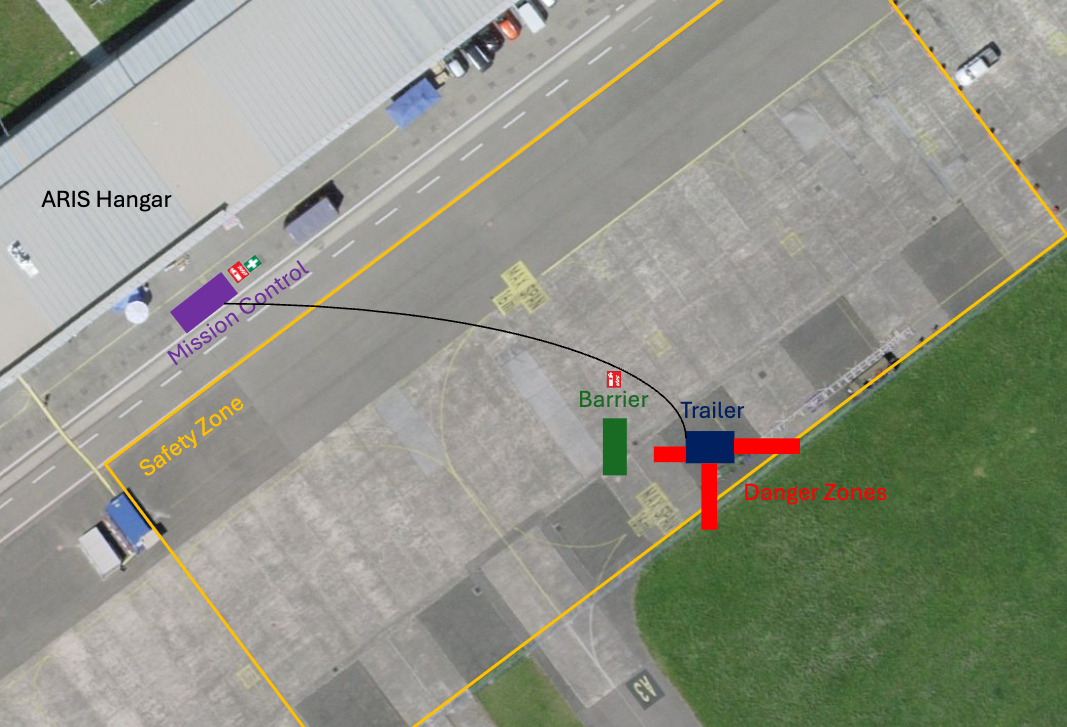
\includegraphics[width=\textwidth]{assets/location-map.png}
    \caption{Site map of the test location}
    \label{fig:location-plan}
\end{figure}

\newpage
\section{Equipment}
Every person has to wear a warning vest according to their role at all times during testing operations. The color code displayed in table \ref{tab:color-code} is used.
\begin{table}[h]
    \caption{Warning Vest Color Code}
    \label{tab:color-code}
    \begin{tabularx}{0.9\textwidth}{|X|X|X|X|}
        \hline
        \cellcolor{cyan} Test Conductor & \cellcolor{green} Safety Officer & \cellcolor{orange} Engineers in charge (determined in role assignment) & \cellcolor{yellow} Visitors \\ \hline
    \end{tabularx}
\end{table}
The safety equipment is stored inside the ARIS Hangar. The wearing of provided safety equipmentas foreseen in the operating procedures is mandatory.
\begin{table}[h]
    \caption{Safety Equipment}
    \label{tab:safety-equipment}
    \begin{tabularx}{0.9\textwidth}{|c|X|X|}
        \hline
        \rowcolor{tableHeaderColor} \textbf{Amount} & \textbf{Equipment} & \textbf{Comment} \\ \hline
        2 & Fire extinguisher & ABC-Pulver \\ \hline
        2 & Fire extinguisher & CO2 (class B next to trailer) \\ \hline
        1 & First aid kit &  \\ \hline
        2 & Blue warning vest & \\ \hline
        2 & Green warning vest & \\ \hline
        10 & Yellow warning vest & \\ \hline
        6 & Orange warning vest & \\ \hline
        8 & Safety goggles & \\ \hline
        4 & Face shield & \\ \hline
        2 & Cold-resistant gloves & For handling LOX \\ \hline
        1 & Cryogenic apron & \\ \hline
        6 & Pair of safety shoes & \\ \hline
        10 & Ear protection & \\ \hline
        8 & Work gloves & \\ \hline
        2 & Barrier tape & \\ \hline
    \end{tabularx}
\end{table}
\section{Behaviour during test procedure}
The test conductor has the lead during the whole test operation and therefore gives the orders, which shall be obeyed. The safety officer supervises the actions of the test conductor and the team and makes sure that the tests are executed according to the procedures. The safety officer can stop the operations at any time he considers proceeding with the test as dangerous. \\
\noindent
If during the test procedure an anomaly occurs or if there is an insecurity, the test participants are requested to inform the test conductor and the safety officer immediately.
\newpage
\section{Behaviour in case of an emergency} \label{emergency-behaviour}
In case of an emergency or an unexpected system state, the contingency procedures (shown in table \ref{tab:contingency-procedures}) must be followed. Participants will be informed about the location of the contingency procedures during the briefing and installation.
\begin{table}[h]
    \caption{Contingency Procedures}
    \label{tab:contingency-procedures}
    \begin{tabularx}{0.9\textwidth}{|X|}
        \cellcolor{blue} \textcolor{white}{General} \\ \hline
        HEP\_CP\_GEN\_Injury\_XX \\ \hline
        HEP\_CP\_GEN\_Fire\_XX \\ \hline
        HEP\_CP\_GEN\_Trespassing\_XX \\ \hline
        \cellcolor{orange} PSS \\ \hline
        HEP\_CP\_PSS\_Leakage\_XX \\ \hline
        HEP\_CP\_PSS\_Overpressure\_XX \\ \hline
        HEP\_CP\_PSS\_BottleValveAnomaly\_XX \\ \hline
        HEP\_CP\_PSS\_NoisesHissing\_XX \\ \hline
        \cellcolor{yellow} DACS \\ \hline
        HEP\_CP\_DACS\_PowerLoss\_XX \\ \hline
        HEP\_CP\_DACS\_ConnectionLoss\_XX \\ \hline
        HEP\_CP\_DACS\_ValveAnomalies\_XX \\ \hline
    \end{tabularx}
\end{table}
All attendees are guided to stay calm and to avoid panicking. In such a situation, communication needs to be reduced to the minimum / essential only. The safety officer or his substitute leads through all emergency situations supported by the test conductor. \\
\noindent
In any situation, the hazards must be considered before providing assistance.
\noindent
As soon as the situation allows it, the safety officer will inform IPZ and Chloé Pilloud (ARIS). 
\end{document}